

For our experiments, we train our autoencoder over the MNIST handwritten digit
dataset. The MNIST dataset is composed of 60000 training images and 10000
testing images Each image is in greyscale, is 28 by 28 pixels in size, and has
a corresponding label ranging from 0 to 9. Thus, the input vector for our
autoencoder has 784 dimensions. We also make use of the denoising criterion
mentioned in \cite{vincent2010stacked}, and for each training image, randomly
corrupt it by setting each pixel to zero with probability 0.25. 

\begin{figure}[h] \centering
	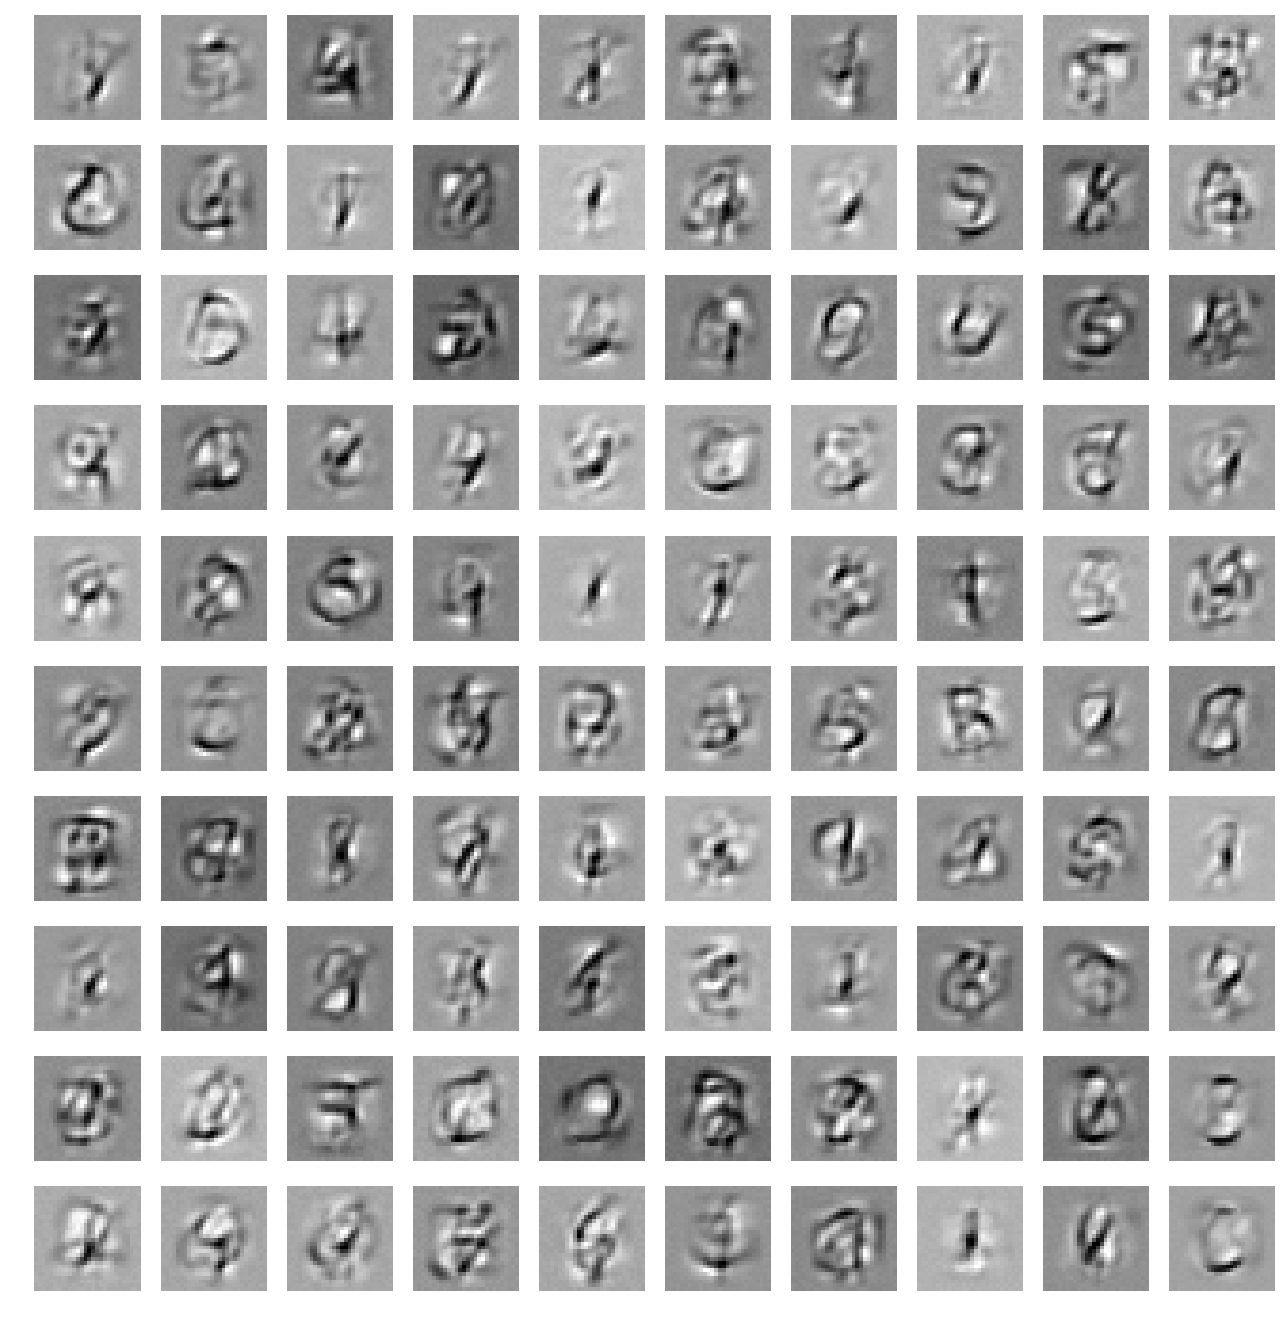
\includegraphics[width=1.0\linewidth]{experiment3_1.png}
	\caption{Visualization of the filters of the first 100 hidden nodes in an
	denoising autoencoder trained over all 60000 images.}
	\label{fig:experiment3_1}
\end{figure}



We first analyze how the number of threads affects the rate at which training
error decreases. We train a single autoencoder layer with 500 hidden nodes for
15 iterations over 5000 training images. An iteration involves going through
all training images and for each image, use SGD to update the weight matrix.
Fig.~\ref{fig:experiment1} shows the relationship between training error, total
time elapsed, and the number of threads used. Regardless of the number of
threads, the training error decreases sharply in the first few iterations
before flattening out to around the same value after 15 iterations. The rate at
which error decreases is significantly faster for four and eight threads when
compared to just using one. Nonetheless, the speedup is not linear and is due
to two reasons: 1) Possible cache conflicts as each thread read and writes to
different locations in the weight matrix. 2) All the steps for
backpropagation/SGD, described in Algorithm \ref{alg:backprop}, must be done
sequentially. Parallelization can only be done within each step and incurs an
overhead cost.


Next, in Fig.~\ref{fig:experiment3_1}, we visualize the filters that are
learned by training an autoencoder layer with 500 hidden nodes over all 60000
training images. The  filter for each hidden node is a row vector of the weight
matrix and indicates which aspects of the input the hidden unit is sensitive
to. Since each row in the weight matrix is the same dimensionality as the
input, we can visualize it as a 28 by 28 pixel image. The filters are not
identical to the input images, but do show some similarity to them. In
Fig.~\ref{fig:reconstruct}, we visualize the reconstructed digits when given
noisy test digits as input. The reconstructed outputs for most of the input
images are easily recognizable as digits, which indicates that the autoencoder
is indeed denoising and learning a good representation of the images.

To further demonstrate the reconstruction capabilities of the autoencoder, we 
trained the autoencoder on corrupted or otherwise altered digits.
In particular, we test the reconstruction
on \textit{bg-rand}, which is generated from the MNIST dataset, excpt that
a random backgound is added. In \textit{bg-img}, each image is given a background
randomly selected from one of twenty images downloaded form the internet. In 
\textit{rot}, the digits are simply rotated by some random angle.
These alterations to the images make the classification task more difficult. Indeed the
digits are very difficult to identify, but the autoencoder creates an easier to identify 
representation, even to the human eye. We show also in Fig.~\ref{fig:reconstruct} 
the reconstructed images form the \textit{bg-img} and \textit{rot} datasets. Note that
the images in the \textit{bg-rand} and \textit{bg-img} datasets are rotated, but they
are all rotated in the same way.



Finally we evaluate the classification accuracy of a deep neural network that
has multiple stacked denoising autoencoders. We train 3 stacked autoencoder
layers, each with 1000 hidden units, and using noise levels 0.1, 0.2, and 0.3
respectively. Each layer is trained for 15 iterations with a learning rate of
0.001. After the unsupervised pretraining, a conventional feedforward network
with 1000 input units, 500 hidden units and 10 outputs is connected to the
hidden units of the last autoencoder layer. This conventional network is then
trained for 30 iterations (learning rate 0.1) in a supervised manner, where the
target $t$ is the indicator vector representation of the training label. Our
final classification accuracy is 98.04\%. In comparison, the accuracy achieved
with a SVM with RBF kernel is 98.60\% \cite{vincent2010stacked}. 


Recall that one of the main reasons for using an autoencoder is to determine a
more useful representation of the data for other tasks, for example in a
classification task. To this end, we constructed and trained (15 iterations) an
autoencoder with just a single layer and 1000 hidden units and used it to
create a more useful representation of the digits in the MNIST dataset. After
this more useful representation is constructed, we can then use the output from
the autoencoder as input to another type of classification algorithm.  Since
the autoencoder produces a better representation of the data, we expect that
given the encoded data, the other classification algorithms should perform
better.  The results of these experiments is given in
Table.~\ref{tab:classvsenc}.


To test this,we used liblinear to attempt to train a model and then predict on
a test set for both the enocded and unencoded datasets. With the original data
liblinear gives an accuracy of 91.68\% on the test set when using the default
parameters. However, when the encoded data from the trained autoencoder gives
an accuracy of 97.07\%. This is a nontrivial improvement in the classification
accuracy. Thus, the autoencoder has created a better representation of the data
which maed it easier for liblinear to classify. This verifies that the
autoencoder is doing what it is expected to do.

Similarly, we performed the same experiment as above, except in this case we
used libsvm with an RBF kernel and all the default parameters.  Without
encoding the data first, we get an accuracy of 94.46\%, but using the encoded
data gives a prediction accuracy of 95.48\%. As above, the encoded data allows libsvm
better classify the data.

Using logistic regression to perform the classification, we experienced similar results.
Again we use liblinear with all default options except selecting logistic regression. Using the
original MNIST data, this algorithm achieved an accuracy of 91.82\% while with the encoded data
we achieved an accuracy of 96.86\%.

\begin{table}[h]
	\begin{tabular}{l|lll}
		& Linear SVM & Kernel SVM (RBF) & Logistic Regression \\ \hline
		Original & 91.68\%    & 94.46\%          & 91.82\%             \\
		Encoded  & 97.07\%    & 95.48\%          & 96.86\%            
	\end{tabular}
	\label{tab:classvsenc}
	\caption{Summary of the results of running different classifcation algorithms on the raw MNIST data and on the output from a trained autoencoder. We
	see in all cases that using the encoded data produces a better result.}
\end{table}

\subsection{Training the AE with a GA}




